\begin{theorem}[Query Complexity]
The number of comparisons to answer a $d$-dimensional query is $2^d-1$.
\end{theorem}
\emph{Proof:} With the preprocessed data structure any online query can be divided into $2^d$ subqueries each of which can be answered directly from $DominanceMin$ structure of some $CR$ without any comparison. And $d$ Nearest Common Ancestor query is enough to find out $2^d$ $CR$s. Therefore $2^d-1$ comparison is sufficient to answer any Range Minimum Query.
\section{Implementation in RAM Model}
\section{Micro Data Structure}
The key idea is to divide the input array into micro-blocks with the following properties. 
\compress
\begin{itemize}\topsep0pt \itemsep1pt \parskip0pt \parsep0pt
\item Each dimension of $d$-dimensional microcube is $g=(\epsilon\log N)^{1/d}$, size $G=\epsilon\log N$.
\item Type of a microblock is a sequence of comparison results ($0/1$) from the linear-time preprocessing algorithm. Micro-blocks with same type share same data structure.
\item It takes $B(d)\epsilon\log N$ comparison to preprocess a block and it is so chosen that $\epsilon < \frac{1}{B(d)}$, therefore total no of distinct micro-block types is $2^{B(d)\epsilon\log N} = N^{B(d)\epsilon} = N^f$ where $f < 1$, implies \emph{sublinear}.
\item Types can be recognized using linear-depth ($B(d)G$) decision tree according to the preprocessing algorithm.
\end{itemize}
\section{Decision Tree: Indices Structure ($1D$)}
The key idea here is to store indices of the minimum element for each type of microblock for all possible queries instead of the actual element. This greatly reduces both the space and time complexity of the algorithm, as the number of distinct micro-block type is sublinear. Let's say $PosLeftMin(I,x)$ and $PosRightMin(I,x)$ calculates indices of $LeftMin$ and $RightMin$. Now a structure called $Indices(t,q)$ stores these candidates for each query and $Indices(t,q)[i]$ where $0\leq i\leq1$ is the index of $i^{th}$ such candidate for query $q$ in type $t$ micro-block. The tree has the following properties
\compress
\begin{itemize}\topsep0pt \itemsep1pt \parskip0pt \parsep0pt
\item It is similar to a deterministic program that accepts size of input array and is allowed to call a compare function but can not access elements in the input directly
\item Each internal tree node holds a program state, i.e. a comparison function with indices for the array entries to compare.
\item Root stores $PosLeftMin(I(x),x) = x$,$PosRightMin(I(x),x) = x$ $\forall$ $1\leq x\leq g$ and canonical interval $[x,x]$.
\item Each leaf of the decision tree contains a configuration representing the halting state of the program, that is the Indices structure.
\item Two children of each node represent results of comparison
\item Path from root to any leaf corresponds to a micro-block type
\end{itemize}
\begin{lemma}
The total time and space (in terms of bits) complexities for constructing the micro data structures are $\mathcal{O}(B(d)N)$.
\end{lemma}
\emph{Proof:} Total no. of decision tree nodes is $\mathcal{O}(2^{B(d)G})$, each node costs $\mathcal{O}(G\log^dG)$ time and $\mathcal{O}(G\log^{d+1}G)$ bits space, therefore total complexity is $\mathcal{O}(2^{B(d)G}\cdot G\log^{d+1}G)$. $Indices$ structure costs a total $\mathcal{O}(2^{B(d)G}\cdot G^2)$ time and $\mathcal{O}(2^{B(d)G}\cdot G^2\log G)$ bits. Each microcube type can recognized by walking down the entire depth of the tree therefore $\mathcal{O}(B(d)G)$ and can also be stored using $\mathcal{O}(B(d)G)$ bits. Now $B(d)G<B(d)\epsilon\log N<\log N$, so total space for $\frac{N}{G}$ microcubes is $\mathcal{O}(N/G\cdot B(d)G)=\mathcal{O}(B(d)N)$. Therefore, total complexity of building micro-data structure is $B(d)N+2^{B(d)G}G^2 \leq B(d)N+2^{B(d)\epsilon\log N}(\epsilon\log N)^2 = \mathcal{O}(B(d)N)$.

\section{2D Micro-block Example}
\begin{center}
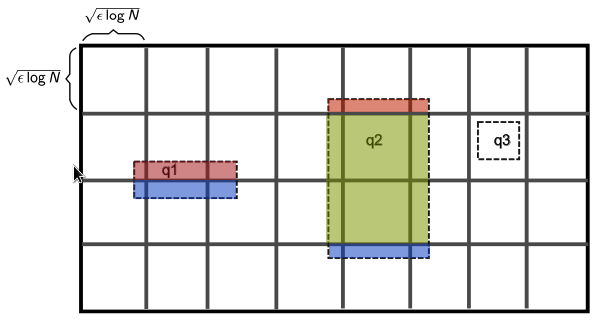
\includegraphics[height=4.5cm,]{img/2dmicro.png}
\end{center}

